\documentclass[11pt]{article}

\usepackage[a4paper]{geometry}
\geometry{left=2.0cm,right=2.0cm,top=2.5cm,bottom=2.5cm}

\usepackage{ctex} % 支持中文的LaTeX宏包
\usepackage{amsmath,amsfonts,graphicx,subfigure,amssymb,bm,amsthm,mathrsfs,mathtools,breqn} % 数学公式和符号的宏包集合
\usepackage{algorithm,algorithmicx} % 算法和伪代码的宏包
\usepackage[noend]{algpseudocode} % 算法和伪代码的宏包
\usepackage{fancyhdr} % 自定义页眉页脚的宏包
\usepackage[framemethod=TikZ]{mdframed} % 创建带边框的框架的宏包
\usepackage{fontspec} % 字体设置的宏包
\usepackage{adjustbox} % 调整盒子大小的宏包
\usepackage{fontsize} % 设置字体大小的宏包
\usepackage{tikz,xcolor} % 绘制图形和使用颜色的宏包
\usepackage{multicol} % 多栏排版的宏包
\usepackage{multirow} % 表格中合并单元格的宏包
\usepackage{pdfpages} % 插入PDF文件的宏包
\RequirePackage{listings} % 在文档中插入源代码的宏包
\RequirePackage{xcolor} % 定义和使用颜色的宏包
\usepackage{wrapfig} % 文字绕排图片的宏包
\usepackage{bigstrut,multirow,rotating} % 支持在表格中使用特殊命令的宏包
\usepackage{booktabs} % 创建美观的表格的宏包
\usepackage{circuitikz} % 绘制电路图的宏包
\usepackage{caption}
\captionsetup{font=normalsize,skip=2pt}

\definecolor{dkgreen}{rgb}{0,0.6,0}
\definecolor{gray}{rgb}{0.5,0.5,0.5}
\definecolor{mauve}{rgb}{0.58,0,0.82}
\lstset{
  frame=tb,
  aboveskip=3mm,
  belowskip=3mm,
  showstringspaces=false,
  columns=flexible,
  framerule=1pt,
  rulecolor=\color{gray!35},
  backgroundcolor=\color{gray!5},
  basicstyle={\small\ttfamily},
  numbers=none,
  numberstyle=\tiny\color{gray},
  keywordstyle=\color{blue},
  commentstyle=\color{dkgreen},
  stringstyle=\color{mauve},
  breaklines=true,
  breakatwhitespace=true,
  tabsize=3,
}

% 轻松引用, 可以用\cref{}指令直接引用, 自动加前缀. 
% 例: 图片label为fig:1
% \cref{fig:1} => Figure.1
% \ref{fig:1}  => 1
\usepackage[capitalize]{cleveref}
% \crefname{section}{Sec.}{Secs.}
\Crefname{section}{Section}{Sections}
\Crefname{table}{Table}{Tables}
\crefname{table}{Table.}{Tabs.}

\setmainfont{Palatino_Linotype}[
  Path = ../Fonts/,
  Extension = .ttf
]
\setCJKmainfont{SimHei}[
  Path = ../Fonts/,
  Extension = .ttf
]
\punctstyle{kaiming}
% 偏好的几个字体, 可以根据需要自行加入字体ttf文件并调用

\renewcommand{\emph}[1]{\begin{kaishu}#1\end{kaishu}}

%改这里可以修改实验报告表头的信息
\newcommand{\studentNum}{00000000}
\newcommand{\name}{我是谁}
\newcommand{\exDate}{2025.04.22}
\newcommand{\weekDay}{二}
\newcommand{\ap}{下午}
%%%%%%%%%%%%%%%%%%%%%%%%%%%

\begin{document}

%若需在页眉部分加入内容, 可以在这里输入
% \pagestyle{fancy}
% \lhead{\kaishu 测试}
% \chead{}
% \rhead{}

\begin{center}
    \LARGE \bf 《\, 基\, 础\, 物\, 理\, 实\, 验\, 》\, 实\, 验\, 报\, 告
\end{center}

\begin{center}
    \emph{学号}\underline{\makebox[6em][c]{\studentNum}}
    \emph{姓名}\underline{\makebox[6em][c]{\name}} 
    \emph{实验日期} \underline{\makebox[8em][c]{\exDate}}
    \emph{星期} \underline{\makebox[2em][c]{\weekDay}}\;\underline{\makebox[3em][c]{\ap}}
    {\noindent}
    \rule[8pt]{17cm}{0.2em}
\end{center}

\begin{center}
    \Large \bf 干涉法测微小量
\end{center}

\section*{一、实验目的}

\begin{enumerate}
    \item 学习光的干涉原理及其应用
    \item 应用等厚干涉原理测量牛顿环的曲率半径;测量细丝直径
\end{enumerate}

\section*{二、实验原理}

\begin{wrapfigure}{r}{5cm}
    \centering
    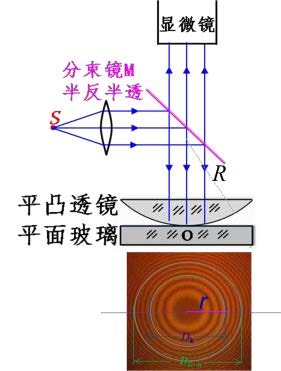
\includegraphics[width=4cm]{Figs/牛顿环结构及光路图.jpg}
    \caption{\small 牛顿环结构及光路图}
\end{wrapfigure}

1. 用牛顿环测平凸透镜的曲率半径

当曲率半径很大的平凸透镜的凸面放在一平面玻璃上时,见图$1$,在透镜的凸面与平面之间形成一个从中心$O$向四周逐渐增厚的空气层。当单色光垂直照射下来时,从空气层上下两个表面反射的光束$1$和光束$2$在上表面相遇时产生干涉。因为光程差相等的地方是以$O$点为中心的同心圆,因此等厚干涉条纹也是一组以$O$点为中心的明暗相间的同心圆,称为牛顿环。由于从下表面反射的光多走了二倍空气层厚度的距离,以及从下表面反射时,是从光疏介质到光密介质而存在半波损失,故$1$、$2$两束光的光程差为
\begin{align}
    \Delta=2\delta+\dfrac{\lambda}{2}
\end{align}
式中$\lambda$为入射光的波长,$\delta$是空气层厚度,空气折射率$n\approx1$。

当光程差$\Delta$为半波长的奇数倍时为暗环,若第$m$个暗环处的空气层厚度为 $\delta_m$,则有
\begin{align}
    \Delta=2\delta_m+\dfrac{\lambda}{2}=(2m+1)\dfrac{\lambda}{2},m=0,1,2,\cdots
\end{align}
$$
\delta_m=\dfrac{m\lambda}{2}
$$
由图1中的几何关系$R^2=r_m^2+(R-\delta_m)^2$,,以及一般空气层厚度远小于所使用的平凸透镜的曲率半径$R$,即$\delta_m<<R$,可得
\begin{align}
    \delta_m=\dfrac{r_m^2}{2R}
\end{align}
式中$r_m$是第$m$个暗环的半径。由式$(2)$和式$(3)$可得
\begin{align}
    r_m^2=mR\lambda
\end{align}
可见,我们若测得第$m$个暗环的半径$r_m$便可由已知$\lambda$求$R$,或者由已知$R$求$\lambda$了。但是,由于玻璃接触处受压,引起局部的弹性形变,使透镜凸面与平面玻璃不可能很理想的只以一个点相接触,所以圆心位置很难确定,环的半径$r_m$也就不易测准。同时因玻璃表面的不洁净所引入的附加程差,使实验中看到的干涉级数并不代表真正的干涉级数$m$。为此,我们将式$(4)$作一变换,将式中半径$r_m$换成直径$D_m$,则有
\begin{align}
    D_m^2=4mR\lambda
\end{align}
对第$m+n$个暗环有
\begin{align}
    D_{m+n}^2=4(m+n)R\lambda
\end{align}
将$(5)$和$(6)$两式相减,再展开整理后有
\begin{align}
    R=\dfrac{D_{m+n}^2-D_m^2}{4n\lambda}
\end{align}
可见,如果我们测得第$m$个暗环及第$m+n$个暗环的直径$D_m$、$D_{m+n}$,就可由式$(7)$计算透镜的曲率半径$R$。

\begin{wrapfigure}{r}{5cm}
    \centering
    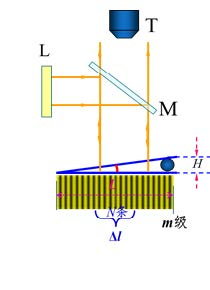
\includegraphics[width=5cm]{Figs/空气劈尖结构及光路图.jpg}
    \caption{\small 空气劈尖结构及光路图}
\end{wrapfigure}

2. 劈尖的等厚干涉测细丝直径

如图$2$所示,两片叠在一起的玻璃片,在它们的一端夹一直径待测的细丝,于是两玻璃片之间形成一空气劈尖。当用单色光垂直照射时,如前所述,会产生干涉现象。因为光程差相等的地方是平行于两玻璃片交线的直线,所以等厚干涉条纹是一组明暗相间、平行于交线的直线。

设入射光波为$\lambda$,则由式$(2)$得第$m$级暗纹处空气劈尖的厚度
\begin{align}
    d=\dfrac{m\lambda}{2}
\end{align}
由式$(8)$可知$m=0$时,$d=0$,即在两玻璃片交线处,为零级暗条纹。如果在细丝处呈现$m=N$级条纹,则待测细丝直径$d=\dfrac{N\lambda}{2}$。

具体测量时,常用劈尖盒,盒内装有两片叠在一起玻璃片,在它们的一端夹一细丝,于是两玻璃片之间形成一空气劈尖,见图$2$。使用时木盒切勿倒置或将玻璃片倒出,以免细丝位置变动,给测量带来误差。

\section*{三、实验仪器}

干涉显微镜、钠光光源、牛顿环、劈尖。

\section*{四、实验内容}

\begin{enumerate}
    \item 测平凸透镜的曲率半径
    \begin{enumerate}
        \item 观察牛顿环
        
        将牛顿环仪放置于载物台上,调节读数显微镜使得牛顿环清晰,观察牛顿环。
        \item 测牛顿环直径
        
        用读数显微镜依次读取牛顿环左右两边第$5$环到第$30$环的直径位置,旋转牛顿环仪,测量三组,各环直径取平均。
        \item 用逐差法处理数据
        
        第30环的直径$D_{30}=d_{30}-d_{30}^'$,同理,可求出$D_{25}$、$D_{20}$、$\cdots$、$D_5$,式$(7)$中,取$n=15$,求出$(D_{m+15}^2-D_m^2)$。代入式$(7)$计算$R$的平均值和标准差。
    \end{enumerate}
    \item 测细丝直径
    \begin{enumerate}
        \item 将劈尖盒放置于载物台上,调节读数显微镜,观察到干涉条纹,使条纹最清晰;
        \item 在劈尖的三个不同部位,用读数显微镜测$20$条暗纹的距离$\Delta l$,测三次求其平均值以及单位长度的干涉条纹数$n=\dfrac{20}{\Delta l}$;
        \item 求细丝直径
        \begin{align}
            d=L\cdot\dfrac{20}{\Delta l}\cdot\dfrac{\lambda}{2}
        \end{align}
    \end{enumerate}
\end{enumerate}

\section*{五、数据记录}

原始数据见附页。

\section*{六、数据处理}

\begin{enumerate}
    \item 牛顿环曲率半径的计算
    
    计算$D_n$

    第一次:
    \begin{align*}
        D_{30}&=d_{30}-d_{30}^'=28.95\,mm-20.99\,mm=7.96\,mm \\
        D_{25}&=d_{25}-d_{25}^'=28.61\,mm-21.32\,mm=7.29\,mm \\
        D_{20}&=d_{20}-d_{20}^'=28.24\,mm-21.68\,mm=6.56\,mm \\
        D_{15}&=d_{15}-d_{15}^'=27.82\,mm-22.10\,mm=5.74\,mm \\
        D_{10}&=d_{10}-d_{10}^'=27.34\,mm-22.59\,mm=4.75\,mm \\
        D_5&=d_5-d_5^'=26.73\,mm-23.21\,mm=3.52\,mm
    \end{align*}

    第二次:
    \begin{align*}
        D_{30}&=d_{30}-d_{30}^'=28.93\,mm-20.97\,mm=7.96\,mm \\
        D_{25}&=d_{25}-d_{25}^'=28.61\,mm-21.31\,mm=7.30\,mm \\
        D_{20}&=d_{20}-d_{20}^'=28.24\,mm-21.67\,mm=6.57\,mm \\
        D_{15}&=d_{15}-d_{15}^'=27.82\,mm-22.08\,mm=5.74\,mm \\
        D_{10}&=d_{10}-d_{10}^'=27.34\,mm-22.57\,mm=4.77\,mm \\
        D_5&=d_5-d_5^'=26.71\,mm-23.17\,mm=3.54\,mm
    \end{align*}

    第三次:
    \begin{align*}
        D_{30}&=d_{30}-d_{30}^'=28.96\,mm-20.99\,mm=7.97\,mm \\
        D_{25}&=d_{25}-d_{25}^'=28.63\,mm-21.32\,mm=7.31\,mm \\
        D_{20}&=d_{20}-d_{20}^'=28.26\,mm-21.69\,mm=6.57\,mm \\
        D_{15}&=d_{15}-d_{15}^'=27.85\,mm-22.10\,mm=5.75\,mm \\
        D_{10}&=d_{10}-d_{10}^'=27.36\,mm-22.58\,mm=4.78\,mm \\
        D_5&=d_5-d_5^'=26.74\,mm-23.20\,mm=3.54\,mm
    \end{align*}

    计算$D_n$的平均值
    \begin{align*}
        \overline{D_{30}}&=\dfrac{7.96+7.96+7.97}{3}\,mm=7.96\,mm \\
        \overline{D_{25}}&=\dfrac{7.29+7.30+7.31}{3}\,mm=7.30\,mm \\
        \overline{D_{20}}&=\dfrac{6.56+6.57+6.57}{3}\,mm=6.57\,mm \\
        \overline{D_{15}}&=\dfrac{5.74+5.74+5.75}{3}\,mm=5.74\,mm \\
        \overline{D_{10}}&=\dfrac{4.75+4.77+4.78}{3}\,mm=4.77\,mm \\
        \overline{D_5}&=\dfrac{3.52+3.54+3.54}{3}\,mm=3.53\,mm
    \end{align*}
    
    取$n=15$,$\lambda=589.3\,nm$,运用逐差法计算$R$的平均值

    \begin{align*}
        \overline{R}&=\dfrac{1}{3}\times\dfrac{\overline{D_{30}}^2-\overline{D_{15}}^2+\overline{D_{25}}^2-\overline{D_{10}}^2+\overline{D_{20}}^2-\overline{D_{5}}^2}{4\times15\times\lambda} \\
        &=\dfrac{(7.96^2-5.74^2+7.30^2-4.77^2+6.57^2-3.53^2)\times10^{-6}\,m^2}{3\times4\times15\times589.3\times10^{-9}\,m} \\
        &=0.864\,m
    \end{align*}

    相对误差为:
    $$
    \dfrac{|\overline{R}-R_{ref}|}{R_{ref}}=\dfrac{|0.864\,m-0.85\,m|}{0.85\,m}\times100\%=1.65\%
    $$

    \item 细丝直径的计算
    
    计算单位长度的干涉条纹数$n$
    \begin{align*}
        n=\dfrac{20}{\Delta l}=\dfrac{20}{2.04\,mm}=9.80\,mm^{-1}
    \end{align*}
    
    取$\lambda=589.3\,nm$,计算细丝直径$d$
    \begin{align*}
        d&=L\cdot\dfrac{20}{\Delta l}\cdot\dfrac{\lambda}{2} \\
        &=L\cdot n\cdot\dfrac{\lambda}{2} \\
        &=35.81\,mm\times9.80\,mm^{-1}\times\dfrac{589.3\times10^{-6}\,mm}{2} \\
        &=0.103\,mm
    \end{align*}
\end{enumerate}

\section*{七、误差分析}

\begin{enumerate}
    \item 读数时连续读数应该估读到精度的后一位,即$0.001\,mm$,但是实验者并没有这么做,只读到了$0.01\,mm$,所以在读数时会有误差。
    \item 玻璃表面有油污或灰尘,会导致某些区域存在附加程差,光程差不等于半个波长。
    \item 牛顿环分布较密集,实验者可能数错环数,造成误差。
    \item 平凸透镜与平面玻璃接触点存在弹性形变,导致理论公式中的$\delta_m=\dfrac{r_m^2}{2R}$与实际值存在偏差。
\end{enumerate}

\section*{八、思考题}

\begin{enumerate}
    \item 如果环的直径测量不准确,对结果有何影响?
    
    答:由公式$R=\frac{D_{m+n}^2-D_m^2}{4n\lambda}$可知,直径误差$\Delta D$将导致$R$的误差$\Delta R \propto 2D\cdot\Delta D$,直径的误差会被平方放大,对结果造成较大影响。

    \item 在干涉法测量微小量的实验中,为什么需要使用单色光源?如果使用白光光源,会对实验结果产生什么影响?
    
    答:因为等厚干涉$\Delta = (2m+1)\frac{\lambda}{2}$,不同波长光的干涉条纹间距不同。白光包含连续光谱,会导致:
    \begin{enumerate}
        \item 高级次条纹因色散重叠而模糊,无法分辨具体环序;
        \item 仅零级附近可见彩色条纹,有效测量范围大幅缩小;
        \item 暗环/亮环边界不清晰,引入主观判断导致的误差;
        \item 计算时无法确定波长,导致无法计算曲率半径和细线直径。
    \end{enumerate}
    因此必须使用单色光源。
\end{enumerate}

\section*{九、实验结论}

利用读数显微镜、钠灯、牛顿环与空气劈尖,通过空气薄膜的等厚干涉测量透镜的曲率半径与两块光学玻璃片所夹细丝的直径,并进行数据处理与误差分析。由上述数据处理可知,待测透镜的曲率半径为$0.864\,m$,待测细丝的直径为$0.103\,mm$。

\end{document}